\usetikzlibrary{backgrounds}

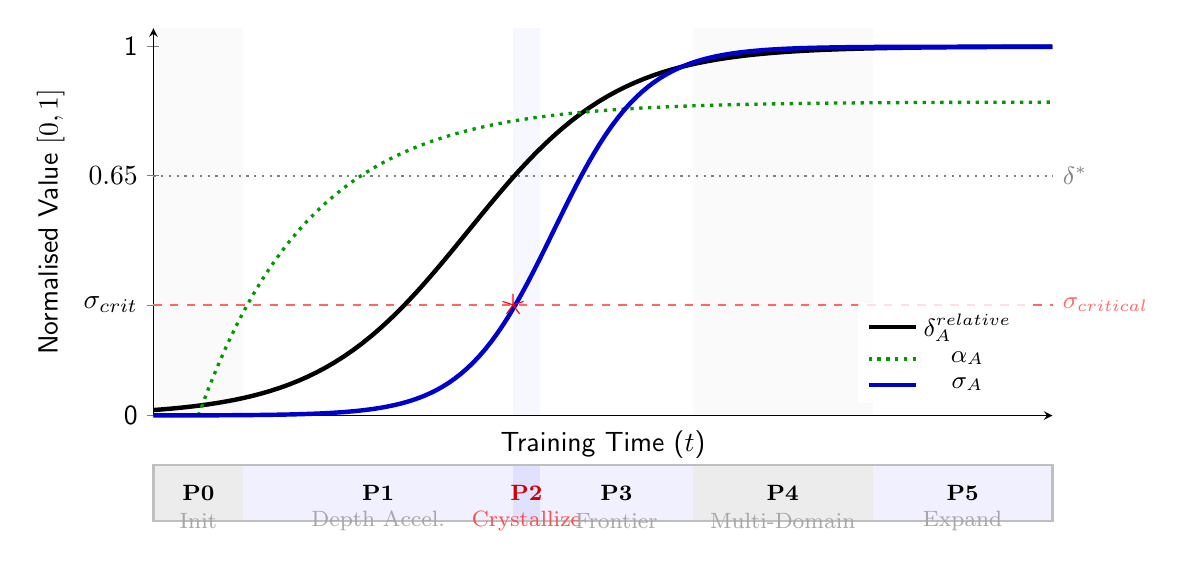
\begin{tikzpicture}[font=\sffamily]
\begin{axis}[
    width=13cm, height=6.5cm,
    xmin=0, xmax=10,
    ymin=0, ymax=1.05,
    xlabel={Training Time ($t$)},
    ylabel={Normalised Value $[0, 1]$},
    xtick=\empty,
    ytick={0, 0.3, 0.65, 1},
    yticklabels={0, $\sigma_{\text{crit}}$, $0.65$, 1},
    axis lines=left,
    legend pos=south east,
    legend style={draw=none, fill=white, fill opacity=0.8, text opacity=1, font=\small},
    clip=false
]

    % Phase Backgrounds
    \begin{scope}[on background layer]
        \fill[gray!4]  (axis cs:0,0) rectangle (axis cs:1,1.05);
        \fill[white]   (axis cs:1,0) rectangle (axis cs:4,1.05);
        \fill[blue!3]  (axis cs:4,0) rectangle (axis cs:4.3,1.05);
        \fill[white]   (axis cs:4.3,0) rectangle (axis cs:6,1.05);
        \fill[gray!4]  (axis cs:6,0) rectangle (axis cs:8,1.05);
        \fill[white]   (axis cs:8,0) rectangle (axis cs:10,1.05);
    \end{scope}

    % Threshold Lines
    \draw[dashed, red!60, thick] (axis cs:0,0.3) -- (axis cs:10,0.3) node[right, font=\small] {$\sigma_{\text{critical}}$};
    \draw[dotted, gray, thick] (axis cs:0,0.65) -- (axis cs:10,0.65) node[right, font=\small] {$\delta^*$};

    % Curves
    % Delta (Depth) - Logistic/Gompertz approximation
    \addplot[domain=0:10, samples=100, ultra thick, black] {1 / (1 + exp(-1.2*(x-3.5)))};
    \addlegendentry{$\delta_A^{\text{relative}}$}

    % Alpha (Attention) - Rises early, then stabilizes
    \addplot[domain=0:10, samples=100, very thick, dotted, green!60!black] {0.85 * (1 - exp(-0.8*(x-0.5))) * (x>0.5)};
    \addlegendentry{$\alpha_A$}

    % Sigma (Schema) - Starts rising in Phase 1, crosses sigma_critical at Phase 2 boundary
    \addplot[domain=0:10, samples=150, ultra thick, blue!80!black]
        {1/(1+exp(-2.0*(x-4.45)))};
    \addlegendentry{$\sigma_A$}

    % Trigger marker (star at sigma_critical crossing)
    \addplot[only marks, mark=star, mark size=4pt, red, mark options={fill=red}] coordinates {(4, 0.3)};

    % Phase Bar (below plot, clean design)
    \begin{scope}[yshift=-18]
        \fill[gray!15] (axis cs:0,-0.15) rectangle (axis cs:1,0);
        \fill[blue!6]  (axis cs:1,-0.15) rectangle (axis cs:4,0);
        \fill[blue!12] (axis cs:4,-0.15) rectangle (axis cs:4.3,0);
        \fill[blue!6]  (axis cs:4.3,-0.15) rectangle (axis cs:6,0);
        \fill[gray!15] (axis cs:6,-0.15) rectangle (axis cs:8,0);
        \fill[blue!6]  (axis cs:8,-0.15) rectangle (axis cs:10,0);
        \draw[gray!50, thick] (axis cs:0,-0.15) rectangle (axis cs:10,0);

        % Phase labels (bold, legible)
        \node[font=\footnotesize\bfseries, text=black] at (axis cs:0.5,-0.075) {P0};
        \node[font=\footnotesize\bfseries, text=black] at (axis cs:2.5,-0.075) {P1};
        \node[font=\footnotesize\bfseries, text=red!80!black] at (axis cs:4.15,-0.075) {P2};
        \node[font=\footnotesize\bfseries, text=black] at (axis cs:5.15,-0.075) {P3};
        \node[font=\footnotesize\bfseries, text=black] at (axis cs:7.0,-0.075) {P4};
        \node[font=\footnotesize\bfseries, text=black] at (axis cs:9.0,-0.075) {P5};
    \end{scope}

    % Phase descriptions below bar (footnotesize >= 8pt for JAIR)
    \begin{scope}[yshift=-30]
        \node[font=\footnotesize, text=gray!70] at (axis cs:0.5,-0.06) {Init};
        \node[font=\footnotesize, text=gray!70] at (axis cs:2.5,-0.06) {Depth Accel.};
        \node[font=\footnotesize, text=red!70] at (axis cs:4.15,-0.06) {Crystallize};
        \node[font=\footnotesize, text=gray!70] at (axis cs:5.15,-0.06) {Frontier};
        \node[font=\footnotesize, text=gray!70] at (axis cs:7.0,-0.06) {Multi-Domain};
        \node[font=\footnotesize, text=gray!70] at (axis cs:9.0,-0.06) {Expand};
    \end{scope}

\end{axis}
\end{tikzpicture}
